\label{sec:Implementation}
This chapter documents the technical realisation of the artefact central to this research. It traces the process from exploratory prototyping to the final, fully functional system and shows how iterative design and engineering choices shaped the artefact's ability to retell tabletop role-playing sessions as comics. First, the development environment of the final artefact is described as a baseline. Second, the minimal viable product (MVP) is presented, followed by lessons learned. Finally, the final artefact is discussed in detail.

To create the artefact for this thesis, an iterative design process was followed alongside an agile development strategy. To increase the chance of success and improve usability, each part of the system was developed and tested separately. This enabled rapid changes and targeted improvements after each test cycle.

Development began with a bare-bones pipeline consisting of three stages applied to the input audio. First, the recorded audio was converted to text with a speech-to-text model. Second, the text was converted to a comic-book script with an LLM. Third, the script was transformed into a comic using an image generation model. This approach yielded the minimal viable product that laid the foundation for the final artefact. The first iteration took a one-shot approach in which each stage simply passed its output to the next, without cleaning, validation, or structural considerations between models.

Testing the MVP surfaced multiple issues that informed the final pipeline. The final pipeline first converts audio to text, then cleans the text via punctuation restoration and diarisation, reconstructing who spoke when. This enriched transcript is provided to an LLM to generate a JSON-based comic script. Each panel has its own structured output, and an adaptive sliding context method lets the model draw on as much of the original transcript as needed. The resulting JSON is then converted by an LLM into prompts for an image generation model. Prompts are rendered with a LoRA-enabled image generator, and the resulting images are assembled into a comic layout.

\section{Development Environment}
Before describing the artefact itself, this section outlines the software and hardware environment used to develop and run the system. Because the artefact relies on several locally hosted AI models, establishing a consistent and capable environment was a crucial prerequisite for successful implementation.

Building and running complex AI pipelines locally requires a wide range of libraries and dependencies, many of which are more stable and better supported on Linux. For this reason, the development environment was set up using WSL2 (Windows Subsystem for Linux) to create a full Ubuntu 24.04.2 LTS environment on a Windows host system. This enabled the use of essential machine learning tools and frameworks while still maintaining compatibility with existing Windows-based workflows. Python (version 3.12.3) served as the primary programming language for all components of the artefact. All libraries that were used can be seen in \ref{tab:core-libraries}.

Running large language models and image generation models locally is computationally demanding, both in terms of memory and processing power. All experiments and development work were performed on a machine equipped with an Nvidia RTX 3080 Ti GPU with 12~GB of VRAM, an Intel i7-9700K CPU with 16 cores, and 64~GB of RAM. These specifications were sufficient for running the models used in this project, though they represent the upper range of consumer-grade hardware. Running the full pipeline reliably requires significant GPU memory and processing capacity. These performance requirements shaped several implementation decisions, particularly around model selection and pipeline optimisation.

\subsubsection*{Core Software Libraries}
The artefact relies on a Python-based ecosystem composed of several key open-source libraries:

\begin{table}[H]
\centering
\caption{Core software libraries used in the artefact}
\label{tab:core-libraries}
\begin{tabular}{|p{3cm}|p{10cm}|}
\hline
\textbf{Library} & \textbf{Purpose} \\
\hline
\texttt{diffusers} & Text-to-image generation using diffusion models via the \texttt{DiffusionPipeline} interface. \\
\hline
\texttt{torch} & Deep learning framework used as the backbone for all model inference. \\
\hline
\texttt{Pillow (PIL)} & Image processing and manipulation, such as loading, editing, and saving generated images. \\
\hline
\texttt{ollama} & Local execution of large language models (LLMs) for generating comic scripts and image prompts. \\
\hline
\texttt{whisper} & Automatic speech recognition (ASR) and audio transcription from recorded sessions. \\
\hline
\texttt{transformers} & Access to Hugging Face models, including token classifiers for punctuation restoration. \\
\hline
\texttt{pyannote.audio} & Speaker diarisation and segmentation of transcribed audio. \\
\hline
\texttt{os}, \texttt{json}, \texttt{re}, \texttt{time} & Standard Python libraries for file handling, data serialisation, regular expressions, and runtime management. \\
\hline
\end{tabular}
\end{table}


\section{MVP Development}
Before creating the final artefact, the MVP was developed as an exploratory prototype. Its purpose was twofold: first, to test whether the concept of converting a tabletop role-playing session into a comic book was feasible at all, and second, to gain practical experience with the challenges of building a multi-model AI pipeline. At this stage, the goal was not quality but functionality: to build an end-to-end system that could transform a small piece of raw audio into a comic book page without human intervention. This prototype then served as the basis for identifying requirements and limitations that shaped the final artefact.

\subsection*{The MVP Pipeline}
The MVP pipeline has 4 steps of processing to go from audio recording to comic book. First, Whisper Turbo transcribes the audio recording to raw text. Then Llama 3.1 converts the text to a comic book script. The script is then processed by Stable Diffusion XL to generate the comic book panels. Finally, the panels are assembled into a comic book format using a custom Python script using the PIL library. The pipeline is shown in figure \ref{fig:MVPpipeline}. The audio recording is a single-track recording of a tabletop role-playing game session of which only the first couple of minutes have been used as that was enough to create one page (6 images). The prompt used for Llama can be seen in listing \ref{lst:MPVLlamaprompt}. This prompt generates a description of the panel art and a line of dialogue or narration for each panel. The output is a JSON array of objects, where each object contains the panel art description and the text. The panel art description is then given to Stable Diffusion XL to generate the image with no other instructions. The text is used as a caption for the image. The images are then assembled into a comic book format using a custom Python script which generates a PDF file with the images and captions.

The prototype was deliberately simple. No intermediate validation, error handling, or data cleaning was performed. Outputs from one stage were passed unchanged to the next. This design allowed rapid iteration and made it easier to observe where the system would fail.

\subsection*{Results and observations}
The MVP successfully generated one page of a comic book from the audio input. Although the output was functional as a comic book, the quality was low. The generated images had no consistency and had a lot of AI artefacts, the text had no link to the image, the text itself was all over the place, and more. Still, the fact that a complete pipeline could run end-to-end with no human intervention demonstrated the core feasibility of the concept. This knowledge, and the discovery of many lessons, directly informed the requirements and design improvements discussed in the next section and ultimately shaped the final artefact.

\begin{lstlisting}[style=jsonstyle, caption={Prompt for Comic Book Script Generation}, label={lst:MPVLlamaprompt}]
You are given a segment of a Dungeons & Dragons session transcript:

Session Content:
{content}

Your task is to transform this into a comic book script, broken down into individual panels.

Each panel must include:
- A detailed visual description suitable for image generation (key: "panel art")
- A line of dialogue or narration (key: "text")

Instructions:
- Structure the output as a JSON array of objects.
- Each object must contain exactly two keys:
- "panel art": A vivid, standalone description of the panel art. Include setting, characters, action, and mood.
- "text": A single line of spoken dialogue or narration. Rephrase as a proper sentence if needed, but keep the meaning true to the original session.
- Process the entire input and split it into as many panels as necessary.
- Do **not** include any additional explanation, commentary, or text outside of the JSON array.

Output only a valid JSON array. Example format:

[
{
    "panel art": "A dimly lit tavern filled with laughing patrons. Magnus, a red-bearded human, clinks mugs with Taco and Merle at a wooden table.",
    "text": "So our story begins with the three of you sitting at this tavern."
},
{
    "panel art": "Close-up of Magnus, his face lit by candlelight, a sheepish grin on his face.",
    "text": "Nobody wants chairs anymore. Everyones into wrought iron now."
}
]
\end{lstlisting}



\begin{figure}[!htp]
	\centering
	\includegraphics[scale=0.1]{images/mvpTTRPGtoComic.png}
	\caption[pipeline for the minimal viable product] {The minimal viable product pipeline}
	\label{fig:MVPpipeline}
\end{figure}

\section{From MVP to Final Artefact}
This section discusses how the MVP informed the development of the final artefact. First, it identifies key limitations revealed during initial testing. Next, it outlines design improvements aimed at addressing these shortcomings. These insights are then translated into a set of formal system requirements that guided the development of the final pipeline. Evaluating the MVP's shortcomings is essential not only for improving the prototype but also for understanding the broader challenges of transforming raw TTRPG audio into a structured retelling.

\subsection{Limitations of the MVP}
The MVP was a success in terms of validating the product idea and gathering valuable knowledge about the product requirements and limitations. In this section, lessons learned are described in detail and it is discussed how these lessons will be implemented in the next iteration of the product.

\subsubsection{Art}
The first thing one might see when looking at the MVP output is the art. The art quality is low, it is not very detailed, the characters are not very expressive and the art style is very inconsistent. There are also a lot of generative AI artefacts, like weird faces and inconsistent human anatomy. Furthermore, all these panels are situated in the same tavern, but there is no consistent setting. All these panels also describe 4 different characters but there is no consistent character design between panels.

\subsubsection{Text}
The text has one obvious flaw of clipping outside of the image which is something that needs to be fixed. Other than that, when reading the text it is noticeable that it is not really character dialogue, but things the players are saying. Some of the text is player-to-player dialogue and not in-character dialogue which is something that needs to be filtered out. The text also does not make any sense in terms of story structure. These are just lines of text.

Looking at the entire transcription of the tabletop role-playing game session it can quickly be seen that there is no structure to the text, making it extremely difficult for an LLM to make anything meaningful out of it. Figure X is an excerpt of the transcript where you can see that it is just a consistent stream of text without any structure. This lack of structure illustrates why raw transcripts are insufficient for later pipeline stages: without segmentation or speaker attribution, LLMs cannot infer narrative flow or character intent.

\subsubsection{Composition}
Another noticeable limitation of the MVP is the visual composition of the panels. Most images were generated from similar camera angles, often defaulting to medium shots or frontal views, which reduced visual variety and narrative impact. Without deliberate framing, lighting choices, or camera perspective, the panels failed to convey mood, pacing, or dramatic tension. This limits the expressive potential of the comic and makes scenes visually repetitive. These issues highlight the need for more explicit compositional control in the image generation stage, including metadata for framing, perspective, and atmosphere.

\subsubsection{Automation and Error Handling}
The MVP was built as a straightforward one-shot pipeline, where each model's output was directly passed into the next without validation or fallback. This approach exposed significant fragility, resulting in the program sometimes crashing during processing. Additionally, there was no progress feedback, making debugging difficult. These limitations made the system unreliable for longer recordings and highlighted the need for validation checks and improved automation in the final artefact.

\subsubsection{Conclusion}
Taken together, these limitations show that producing a coherent retelling involves more than transcription and image generation. It requires structured data, validated intermediate steps, and explicit control over narrative and visual elements.

\subsection{Design Improvements}
In this section, possible solutions are discussed which will be implemented in the next iteration of the product. The goal is to improve the quality of the art, text, and composition of the comic book panels.

\subsubsection{Art}
Stable Diffusion is a pre-trained model that is made to work for any art style; to create a consistent art style you could write an art style prompt; however, this creates issues with the token limit that Stable Diffusion has. The proper way to do this is by using a LoRA (Low-Rank Adaptation). LoRAs are a way to fine-tune a pre-trained model on a specific task or domain. In this case, a LoRA can be trained on a specific art style to create a consistent art style for the comic book panels. This will also allow for more detailed and expressive characters. The LoRA can be trained on a dataset of comic book panels in the desired art style. The LoRA can then be used in Stable Diffusion to generate the comic book panels with the desired art style. However, since training a LoRA is outside the scope of this project, a pre-trained LoRA from civitai.com was used. This also comes with the benefit that any LoRA can be used to generate any art style wanted by the user.

\subsubsection{Character consistency}
To create consistent characters between panels, there are 5 different approaches that can be taken. LoRAs can be used for each character, creating a very consistent character design. This does require each character to have a LoRA trained on it, meaning that you need to have art of the character to start with. This would also mean that the images would be generated with multiple AIs generating images and then having to combine them. 
The second option would be image-to-image reference chaining. With this method you give SDXL a reference image of the character and then generate the panel with the character art as a reference. 

The easiest and least consistent manner would be to use consistent prompting. This means that you give the same prompt for each panel with the character description in it. This will, however, not create a very consistent character as each iteration of the prompt will interpret the prompt differently. This results in many different smaller inconsistencies. This, however, would be a good step if the other methods would be too time-consuming to implement. It would most likely require two iterations of generating the image, one for the character and one for the panel art, as the number of tokens in the prompt would be too high to generate the panel art and character art in one go.

Inpainting is a technique where you alter part of an image so that it fits your desired effect. You select an area of the image and then fill it in with a new image, generated by AI. This gives you a way to control very specific parts of an image and fine-tune an image. Normally this requires a lot of manual work where you have to cut out the area which has to be painted in. However, it would be possible to use computer vision to detect the character in the image and then use that as a mask for the inpainting. This might result in a very good solution, but there are potential issues with multiple characters in the same panel.

Lastly, an option could be using ControlNet. This is a technique where you use pose reference images to control the pose of the character in the image.

In the end, it would most likely be best to use most of the above techniques in combination to create the best possible result. Create a LoRA to have consistent character art, use inpainting to place the art on top of the panel art, and use ControlNet to control the pose of the character. 

\subsubsection{Scene consistency}
In the current comic page of the MVP, each scene is taking place in the same tavern, but the tavern is not consistent between panels. Most solutions given in the previous section on character consistency could be used here as well, however, as there are way more variables possible for locations, creating a LoRA is impossible and would defeat the purpose of using AI. You could, however, let AI create images of a tavern and then use those images as reference materials for future uses of that tavern. This means you need to keep track of scenes and locations so that you can bring back the same panels in later parts of the comic book. Implementing a scene-tracking mechanism to support this was explored during development but could not be completed within the scope and timeframe of this project.

\subsubsection{Text}
To fix the text that is in the panels of the comic books, the first step would be to fix the transcript of the game session. As is always the case with AI: Garbage in is garbage out. Fixing the transcript will also have an effect on the other parts of the comic book, as there will be a clearer structure to the text which can be used in a better way to generate images and create structure between panels. To fix the transcription there are a few steps that need to be taken.

After transcribing the audio recording with Whisper there are 3 steps we can take to increase the usability of the text. First, we need to use a Punctuation and Capitalisation Restoration model to fix the text by adding punctuation and capitalisation to the text. This will make the text more readable and easier to understand. The second step would be to use Speaker Diarisation to identify the different speakers in the text. This will help with knowing who said what at which time and allows for accurate character dialogue. Furthermore, this makes it so that the Game Master can be identified as someone who plays multiple characters. A tool to do this is Pyannote Audio, an open-source toolkit written in Python for speaker diarisation. Lastly, combine the cleaned up Whisper transcription with the speaker diarisation to create a structured text file.

The next step is to then use an LLM to check all the text and identify what is character-to-character and what is player-to-player speech. This creates a clear divide between what does and what does not belong in the comic book. For the Game Master the same thing needs to happen, but then it is required to identify which character they are playing at that moment. Then an LLM would need to convert the text into real sentences which make sense in the context of the scene as something someone in the English language would say.

\subsubsection{Conclusion}
These proposed improvements reveal what the system must/could be capable of to generate meaningful retellings. They also highlight requirements for robustness, structure, and consistency across the pipeline. These insights directly inform the system requirements described in the next section.

\subsection{System Requirements}
\label{sec:SystemRequirements}
Based on the lessons learned from the MVP and the desired features for the final artefact, a set of system requirements has been established. These requirements are divided into functional, non-functional and Constraints categories. The following requirements translate the lessons from the MVP and design explorations into actionable criteria for the final artefact.

\subsubsection{Functional Requirements}
\begin{enumerate}
  \item \textbf{Audio ingestion:} The system accepts a single audio file as input and does not require any additional data.
  \item \textbf{Transcription:} The audio is transcribed into time-stamped text, with punctuation restored and speakers distinguished where possible.
  \item \textbf{Structured transcript:} The transcription output is converted into a structured format containing segment timing, speaker information, and spoken content.
  \item \textbf{Comic script:} Each transcript segment is transformed into a structured description of a comic panel, following a consistent schema with key narrative and visual elements.
  \item \textbf{Prompt rendering:} Panel descriptions are converted into textual prompts suitable for image generation.
  \item \textbf{Image generation:} An image is generated for each panel based on its corresponding prompt.
  \item \textbf{Comic assembly:} The generated panels are assembled into a paginated document with captions and a consistent layout.
  \item \textbf{Automation:} The entire process can be executed through a single command without manual intervention during runtime.
\end{enumerate}

\subsubsection{Non-Functional Requirements}
\begin{enumerate}
  \item \textbf{Offline operation:} The system must run entirely offline, without any network connectivity.
  \item \textbf{Robustness:} Malformed outputs trigger bounded retries rather than stopping the pipeline.
  \item \textbf{Extensibility:} Pipeline components such as the LLM or image generation model can be replaced without major changes to the codebase.
  \item \textbf{Usability:} The system provides progress indicators and uses sensible defaults to minimise required user input.
  \item \textbf{Ethics and privacy:} All processing is performed locally, and no user data leaves the device.
  \item \textbf{Output quality:} Generated images must be at least 1024\,$\times$\,1024 pixels, and the final PDF must meet basic readability and layout standards.
\end{enumerate}

\subsubsection{Constraints}
\begin{itemize}
  \item The system must be runnable without an internet connection.
  \item The system must be runnable on a consumer-grade personal computer with sufficient GPU memory.
  \item The system must be open-source and use freely available artificial intelligence models.
\end{itemize}

\section{The Final Artefact}
Building on the requirements and design considerations discussed in Section~\ref{sec:SystemRequirements}, the final artefact was implemented as a fully automated Python-based system. It takes a single audio file as input and produces a complete comic book as output. Unlike the MVP, which prioritised proof-of-concept over robustness, the final artefact integrates structured data handling, validation checks, and more deliberate control over narrative and visual elements.

\subsection{The Final Pipeline}
In this section, the final pipeline is discussed. The pipeline consists of 5 steps which are all discussed in the following subsections. An overview of the entire pipeline can be seen in figure \ref{fig:FinalPipeline}. Furthermore, in table \ref{tab:mvp-vs-final} the key differences between the MVP and the final artefact are shown. These two graphs serve as a good overview of the entire pipeline and the differences between the MVP and the final artefact.

\begin{figure}[!htp]
	\centering
	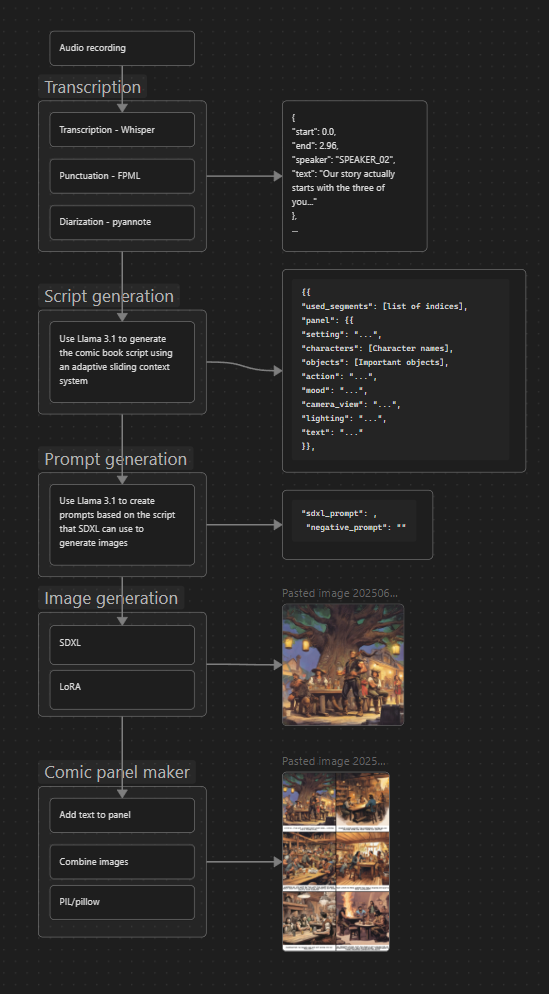
\includegraphics[scale=0.5]{images/FinalPipeLine.png}
	\caption[pipeline for the final artefact] {The final artefact pipeline}
	\label{fig:FinalPipeline}
\end{figure}

\begin{table}[H]
\centering
\small
\caption{Key differences between the MVP and the final artefact}
\label{tab:mvp-vs-final}
\begin{tabular}{|p{3.2cm}|p{5.2cm}|p{5.2cm}|}
\hline
\textbf{Aspect} & \textbf{MVP} & \textbf{Final Artefact} \\
\hline
\textbf{Pipeline design} & Simple one-shot process with raw outputs passed between stages and no validation. & Modular multi-stage pipeline with structured data exchange, validation, and error handling. \\
\hline
\textbf{Data processing} & Audio transcribed into unstructured text without punctuation or speaker information. & Transcription cleaned with punctuation restoration and diarisation, producing structured JSON segments. \\
\hline
\textbf{Script generation} & LLM processed full transcript in one pass, leading to incoherent output. & Adaptive sliding context system with chunking, summarisation, and JSON validation for coherent panel scripts. \\
\hline
\textbf{Visual output} & Image generation lacked style control, consistency, or compositional variety. & LoRA-based style control, metadata for setting, characters, actions, mood, camera view, and lighting. \\
\hline
\textbf{Automation \& usability} & Limited automation, no feedback, and frequent crashes. & Fully automated CLI tool with progress indicators, bounded retries, and minimal user input. \\
\hline
\textbf{Final output} & Single-page comic with basic text overlay. & Multi-page comic with structured layout, captions, and improved readability. \\
\hline
\end{tabular}
\end{table}

\subsubsection*{Transcription}
For clean transcription of a single audio track that has multiple people talking and sometimes through each other, a number of steps had to be taken to turn the audio into usable data. First off, the entire audio recording was transcribed using Whisper. This results in an enormous blob of text with no punctuation and no understandable order of words. Sentences are mixed up, words are missing letters, and many other issues. To clean up this data, two steps had to be taken. First, the audio had to be split up into the different participants. To do this, the diarisation toolkit pyannote.audio was used. This AI model looks at the audio and creates a file with timestamps and speaker, resulting in a file with timestamps that show which speaker speaks at what time. Combining these timestamps with the Whisper output, which also has timestamps, results in data which clearly shows who said what at what time. Lastly, punctuation was restored using the fullstop-punctuation-multilang-large model. This was done so that in the next step it is clear for the LLM what the sentences are. This combination of three different AI models resulted in clean data which can be used in the next step of the pipeline. The output of this step is a structured JSON file with four key-value pairs which can be seen in listing \ref{lst:TranscriptionJSON}.

\begin{lstlisting}[style=jsonstyle, caption={Prompt for Comic Book Script Generation}, label={lst:TranscriptionJSON}]
{
"start": 0.0,
"end": 2.96,
"speaker": "SPEAKER_02",
"text": "Our story actually starts with the three of you..."
}
\end{lstlisting}
\subsubsection*{Script Generation}
To generate the script for the comic book the output of the previous step is given to the large language model Llama 3.1. This model goes through all the data using an adaptive sliding context system. This means that it takes a set number of sentences and then analyses those sentences to see if those can be used to create one panel. The system can respond with 2 different outputs. It has enough data or it needs more data. If the system has enough data it cuts off the data it needs from all the data that it received and uses that to generate a comic book panel script. The data that is not used is fed into the next loop with new data. This means that if in the first loop the system receives sentences 0-50 and uses 0-38, the next loop uses 38-88. If the system outputs that it needs more data, it receives extra sentences, resulting in more context which the model can work with. The usage of this adaptive sliding context system allows for the panel generation to be more coherent and comes with the benefit that there is no loss of data during processing. 

Besides the sentences the AI can use, it also receives a summary of the story so far so that it has more context that it can work with. Context is also why the model did not receive the entire transcript in one go. As Llama 3.1 cannot handle very long text files and will lose understanding of the entire file. Thus this step of giving the model a summary had to be taken so that the model could generate something that was coherent with the entire process.

One of the limitations of Llama 3.1:8B and many other large language models is the context that it can work with. Llama 3.1 has a context limit of 128k tokens which is about 512,000 characters. As we are working with hours of people talking this limit has been exceeded after about 1.5 hours of recording. So to be sure that the system works with any amount of data the input had to be cut up. 

Furthermore, using a lot of context reduces the accuracy and the control over the output. Llama and other language models are known to miss a lot of information when working with a lot of context. A phenomenon often described as being “lost in the middle” \cite{liu2023lostmiddlelanguagemodels}. During testing of the Llama for this step it was found that it is rather bad at outputting proper JSON structure and when asked to output very large files of JSON there is a high chance of failure. Because of this the generation of bite-sized JSON output is better as we can now check the output of each step to see if it is proper JSON and, if not, let the model try again. Because of the nature of LLMs the output is not always correct and thus a test to see if the output is correct had to be done. This testing results in only correct JSON output which can be used in the next step of the pipeline.

The output of this step is a JSON file that can be seen in listing \ref{lst:ScriptGenerationPrompt}.

\begin{lstlisting}[style=jsonstyle, caption={Prompt for Comic Book Script Generation}, label={lst:ScriptGenerationPrompt}]
You are an AI comic scriptwriter adapting a Dungeons & Dragons session.

Here is what has happened so far: {story_so_far.strip()}

Here is the next part of the transcript: {content}

IMPORTANT FILTERING:
- Ignore any rule talk, dice rolls, or out-of-character chatter.
- Focus only on in-character dialogue, world-building, and story-driving actions.
TASK:
Generate ONE new panel based on a selection of lines from this chunk. Your job is to condense meaningful story progression into a single visual scene.
Output JSON in this format:
{{
"used_segments": [list of indices],
"panel": {{
"setting": "...",
"characters": [Character names],
"objects": [Important objects],
"action": "...",
"mood": "...",
"camera_view": "...",
"lighting": "...",
"text": "..."
}},
"summary": "One sentence summary of the panel for story memory."
\end{lstlisting}

\subsubsection*{Prompt Generation}
To create an image generation model prompt that is to be used in the next step, Llama 3.1 is used again. This time the AI is asked to convert each JSON output of the previous step into a prompt that can be fed into Stable Diffusion XL. This step is important as most image generative models work well with human language and not a JSON file. Furthermore, Stable Diffusion has one very large limitation as it can only work with 77 tokens. Of which 2 tokens are reserved as a start and end token. Thus only 75 tokens are available, and that is not a lot. It is unknown how many characters 75 tokens is and how the Stable Diffusion tokenizer works, words can be one token, but certain symbols are also one token. Because of this Llama 3.1 is asked to create a prompt out of the JSON data which is compatible with the 75 token limit. It is asked to create a visually descriptive SDXL prompt based on the JSON output of the previous step. Furthermore, it is given 4 requirements: It should create one natural-language description of the panel image. Use a maximum of 75 tokens. It should not add any other data to the output than the prompt. Lastly it is asked to keep the prompt short and concise so that it sticks within the token limit.

Besides the prompt I have also used the following negative prompt: "deformed, blurry, extra limbs, poorly drawn hands, extra fingers, mutated, out of frame, ugly, tiling, low resolution, bad anatomy, watermark". This negative prompt is used for each image and has its own token limit. The primary reason for this is to increase the image quality without having to spend tokens in the main prompt, but also to prevent strange generative AI artefacts such as multiple limbs.

\subsubsection*{Image Generation}
To generate the images for the comic book the prompt from the previous step is fed into Stable Diffusion XL. Besides this, there are only two other things that are given to the model. The negative prompt that was created is given and a LoRA is passed on to create a consistent art style. A LoRA is a low-rank adaptation of Stable Diffusion which modifies the model in a lightweight way so that you do not have to retrain the whole model. It is similar to fine-tuning. The LoRA used for this project is the Fantasy Art XL LoRA model from Civitai. This LoRA is trained to generate comic book art from the 70s and 80s. With this, the comic book has a coherent art style without having to spend many prompt tokens on the art style. 

\subsubsection*{Comic Book Maker}
Converting all the images to a comic book structure was done with the Pillow Python image library. This is a library which can edit images from Python code. There are 3 steps to take to create a whole comic book. First, the text needs to be added to the image. This was done by adding a white box at the bottom of the image and placing the text inside the white box. I specifically omitted the usage of speech bubbles here because of two things. It would require an extra AI model which uses computer vision to search for faces so we can get an idea of where the speech bubble needs to point towards, which is extra complexity which is outside the scope of this thesis. In addition to that, I assume that this would create a high chance that the speech bubble would overlap with important parts of the image as it would just be placed at random. Normally speech bubbles are part of the artistic vision of the entire panel. The second step is the combining of the images now with text into one page which was also done with the Pillow library. For clarity, a black border was placed between the images. Lastly, all the images had to be combined into one PDF document which was also done with the Pillow library. These 3 steps result in the final resulting comic book.

\section{Chapter Conclusion}
This chapter detailed the development of the artefact which laid the foundation of this thesis, from the creation of a minimal viable product to the implementation of the final system. The MVP demonstrated that generating comic books from tabletop role-playing audio was feasible, but also revealed key limitations around art quality, text structure, composition, and automation. These findings directly informed the system requirements and guided subsequent design improvements.

The final artefact addressed many of these challenges through a structured, multi-stage pipeline, improved data handling, and better control over both narrative and visual elements. It remains a work in progress, but it represents a significant step toward an automated system capable of producing meaningful retellings of TTRPG sessions.

The following chapter evaluates this artefact through both a user-case study and a detailed analysis of its internal data processing, assessing how well it meets its design goals and where further refinement is needed.